\chapter{Ensayos y resultados}

\label{Chapter4}

En este capítulo se describen los ensayos llevados a cabo para verificar que todos los requisitos del proyecto fueron cumplidos.

\section{Ensayos de verificación}

Se ensambló un banco de ensayos para poder evaluar el rendimiento del sistema y resolver los fallos que ocurrieron durante el desarrollo. De esta forma se evitó la dependencia de disponer un motor de combustión interna para los ensayos. Las figuras \ref{fig:banco-pruebas-1} y \ref{fig:banco-pruebas-2} muestran dicho banco de pruebas durante uno de ellos.

\begin{figure}[htpb]
\centering
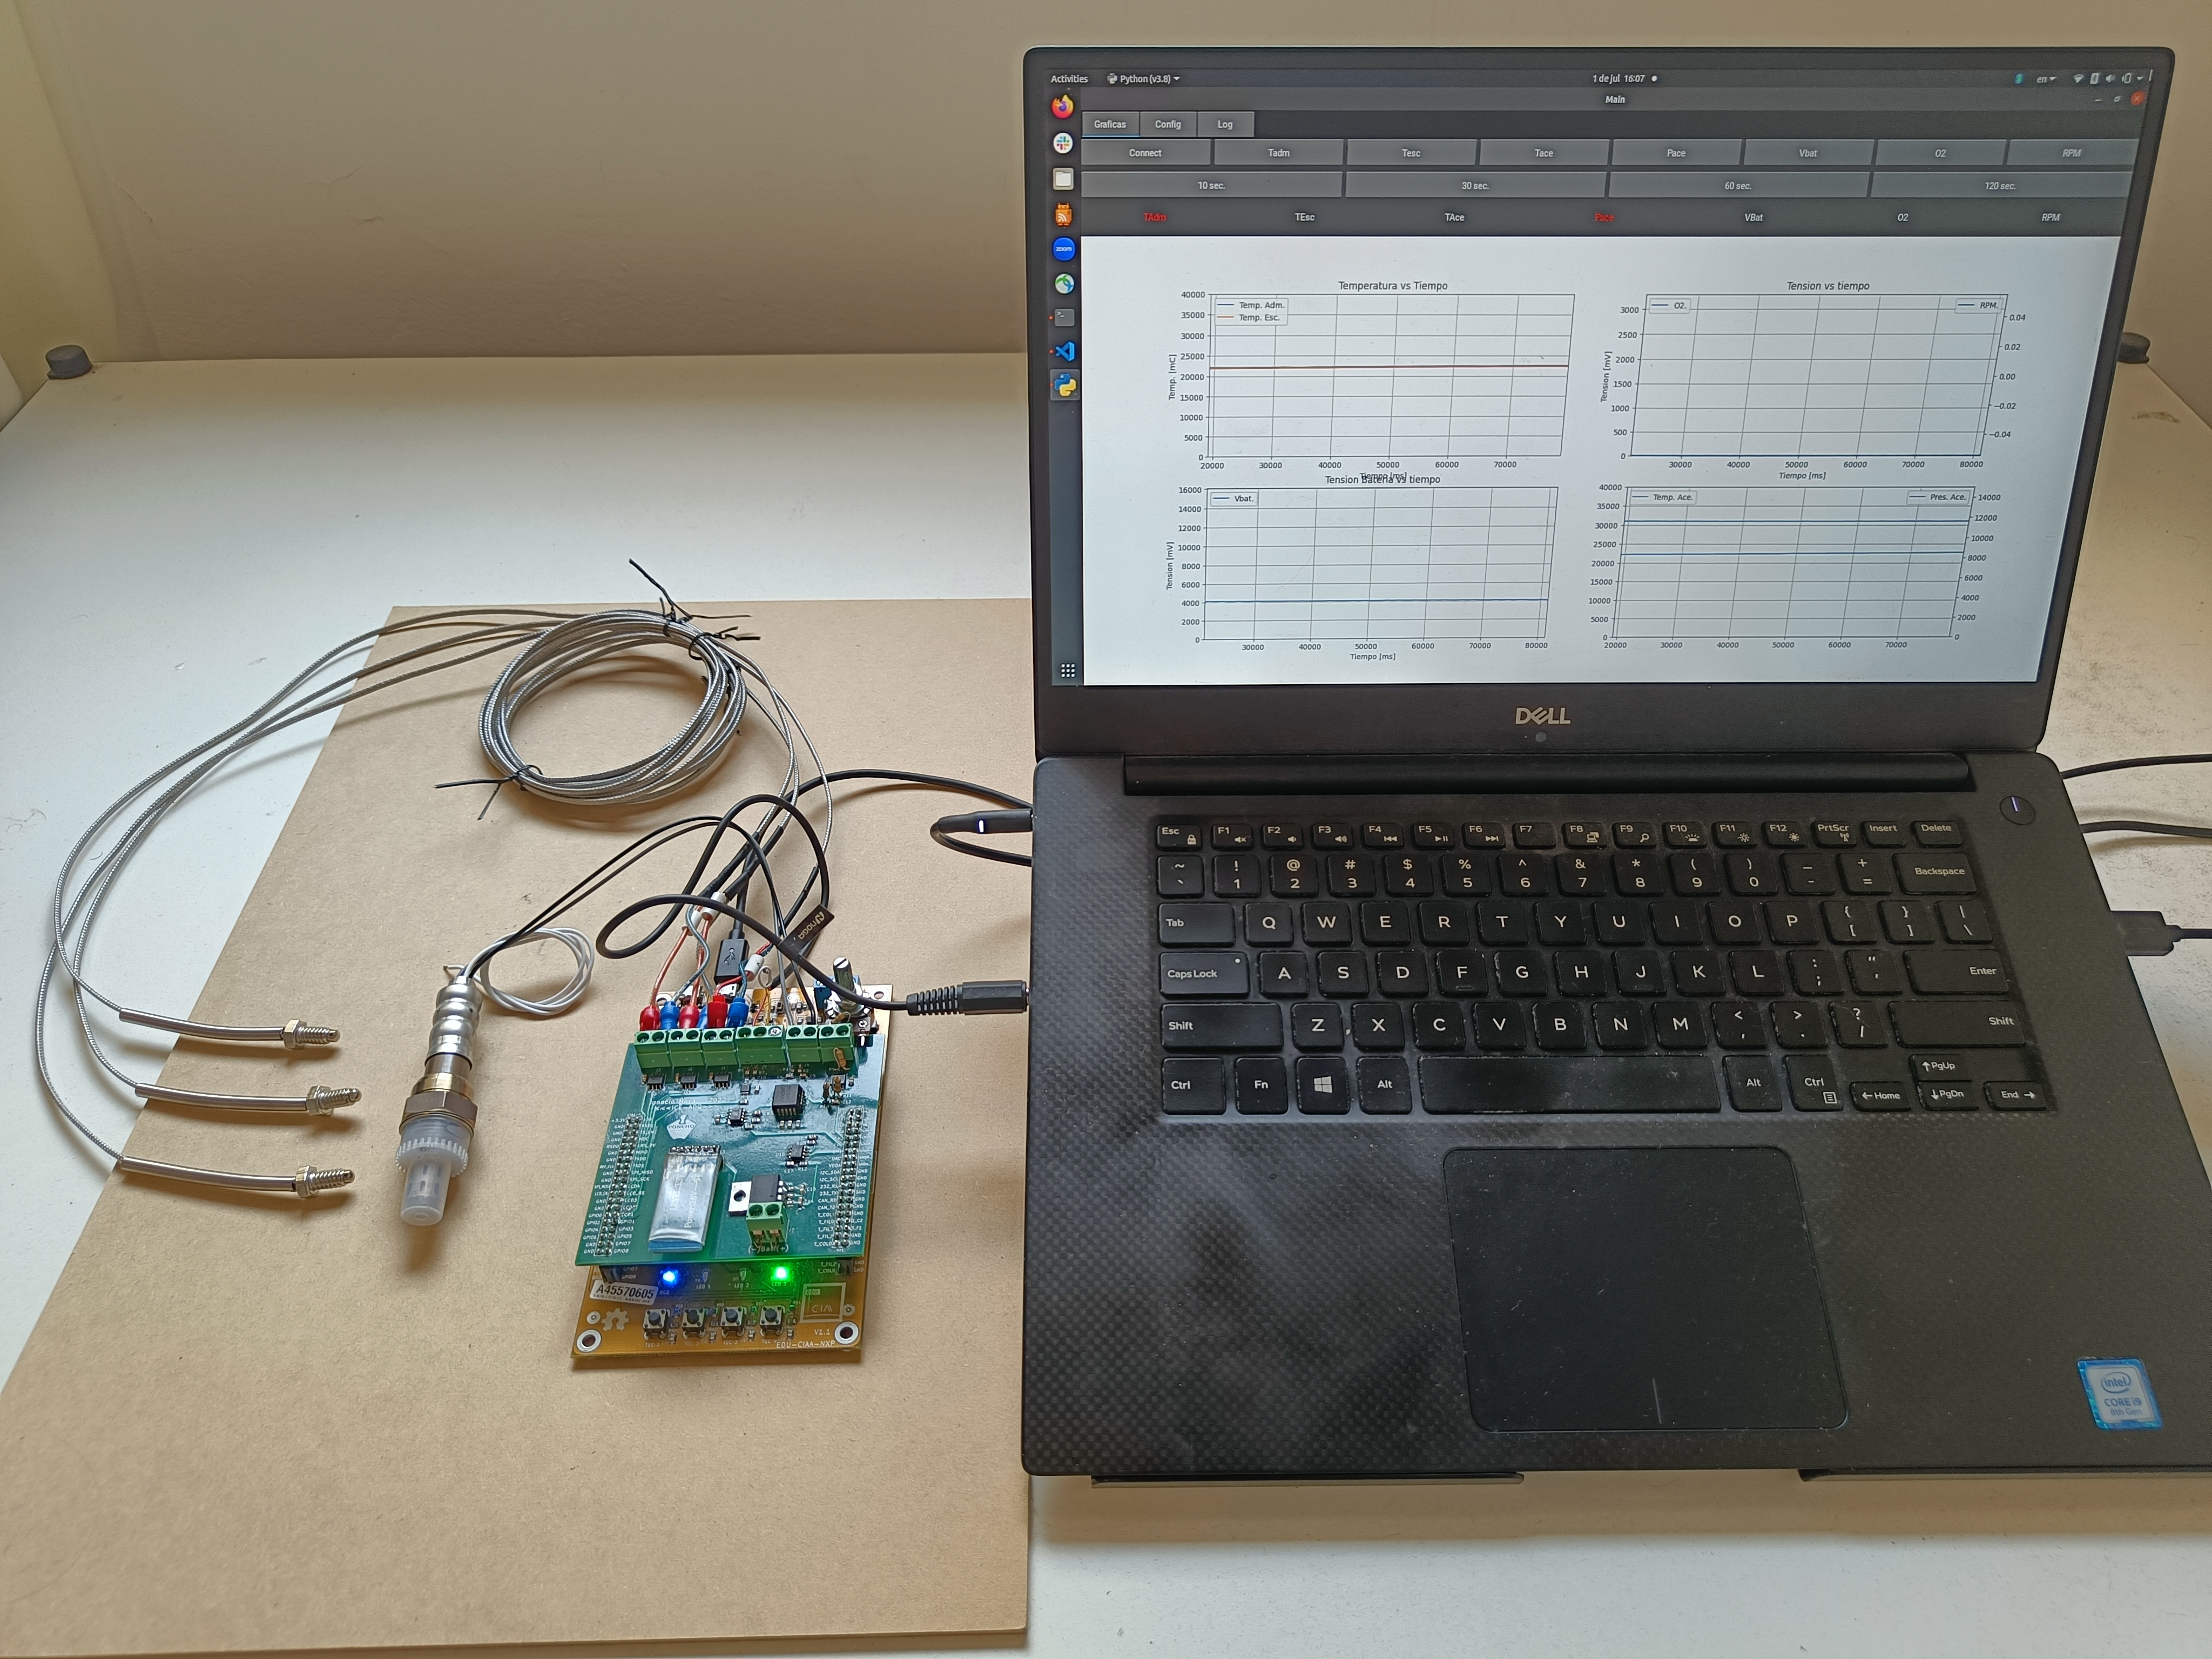
\includegraphics[width=.85\textwidth]{./Figures/banco-pruebas-1.jpg}
\caption{Fotografía del banco de pruebas en uso durante uno de los ensayos.}
\label{fig:banco-pruebas-1}
\end{figure}

\begin{figure}[htpb]
\centering
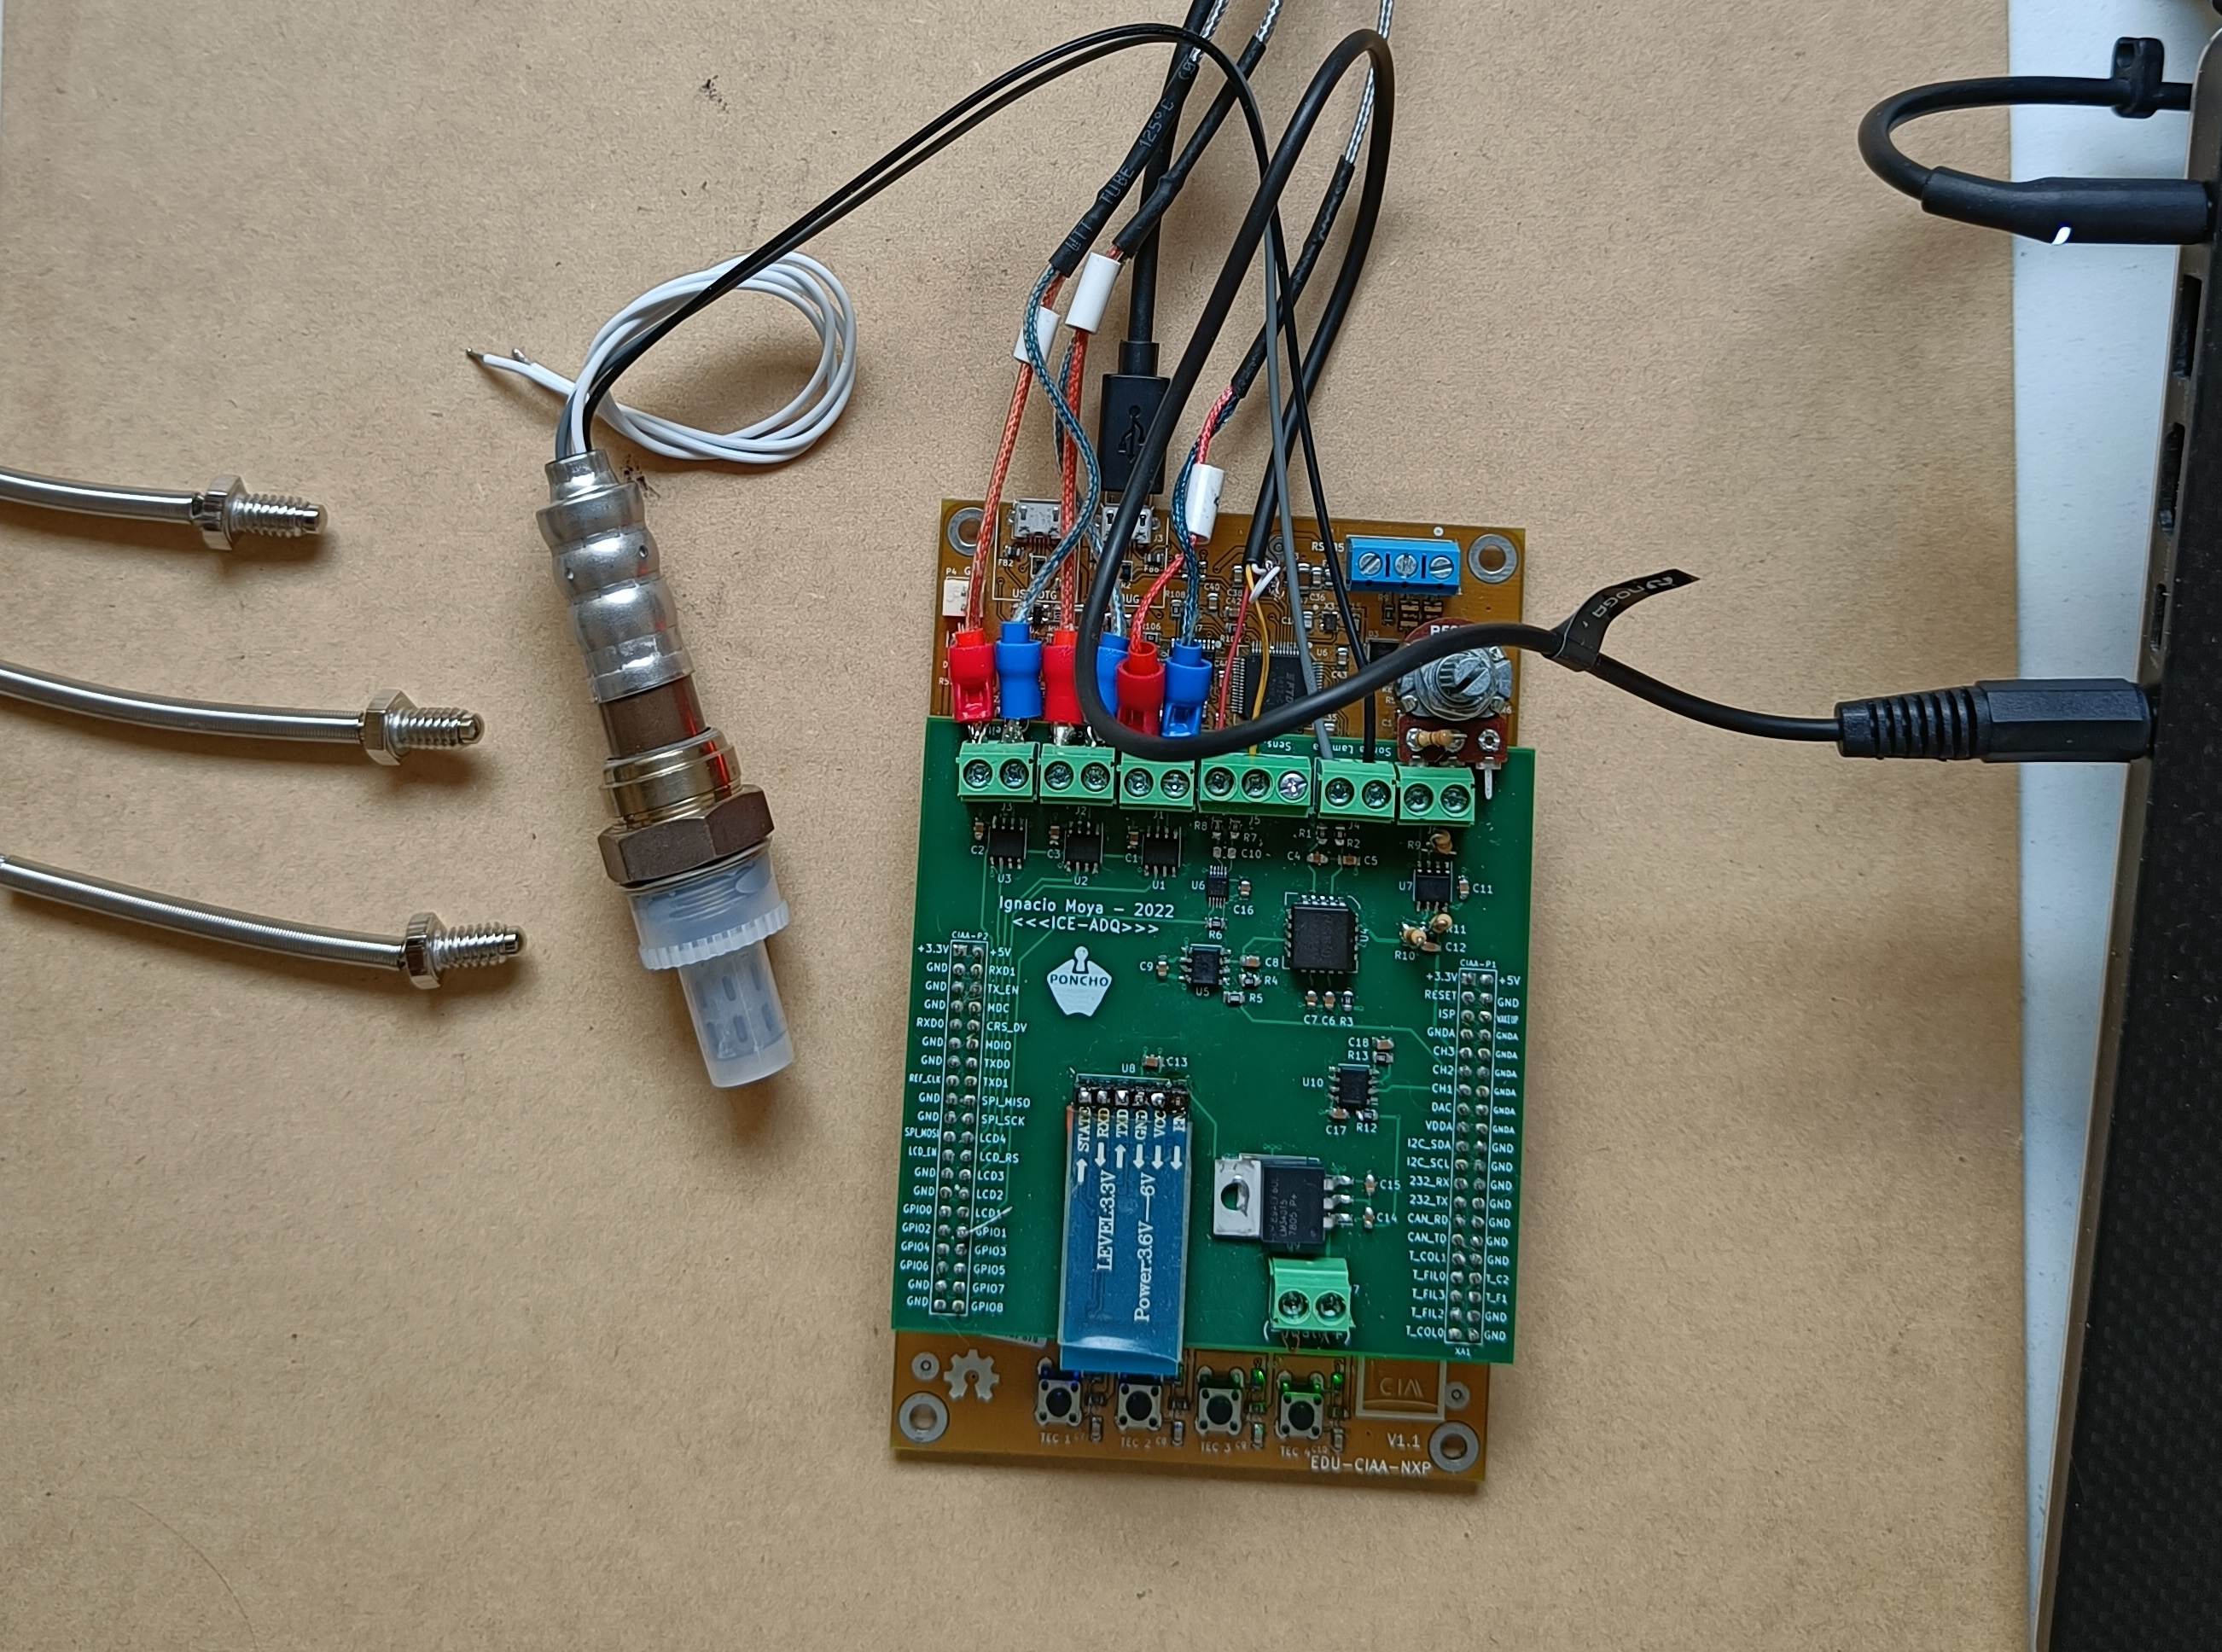
\includegraphics[width=.85\textwidth]{./Figures/banco-pruebas-2.jpg}
\caption{Fotografía en detalle del circuito impreso montado sobre la EDU-CIAA y con sensores conectados.}
\label{fig:banco-pruebas-2}
\end{figure}
\break
\subsection{Ensayos de medición de temperatura}

Se contrastaron las mediciones realizadas por el sistema contra las mediciones realizadas por un multímetro que tiene medición de termocupla tipo K. Para la contrastación se sumergieron a todas las termocuplas en un recipiente con agua, el ensayo se repitió tres veces y en estas reiteraciones la temperatura del agua fue de 0 \degree C, 20 \degree C, considerada temperatura ambiente, y 80 \degree C. Para cada ensayo a cada temperatura se tomaron 150 muestras consecutivas, que representan un tiempo total transcurrido de 375 segundos o 6 minutos 15 segundos. Luego para cada juego de muestras se calculó su valor medio y la desviación estandar, para lograr cuantificar el error y la dispersión que tienen las medidas de temperatura tomadas por el sistema. Estos resultados están plasmados en las figuras \ref{fig:temp-0c}, \ref{fig:temp-20C} y \ref{fig:temp-80c}.

\begin{figure}[htpb]
\centering
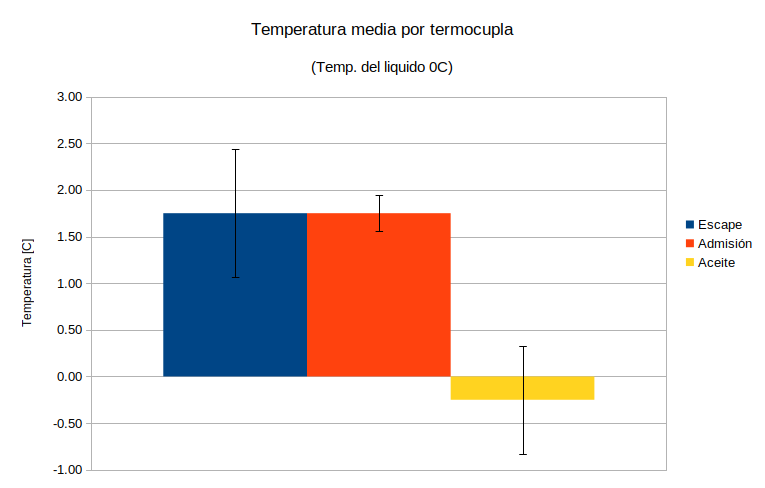
\includegraphics[width=.9\textwidth]{./Figures/temp-0c.png}
\caption{Valores medios y desviación estándar para el ensayo de temperatura a 0C.}
\label{fig:temp-0c}
\end{figure}

\begin{figure}[htpb]
\centering
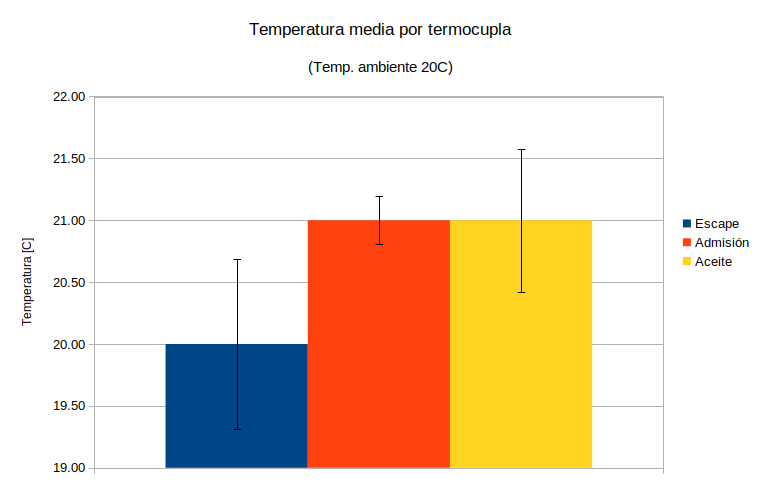
\includegraphics[width=.9\textwidth]{./Figures/temp-20c.png}
\caption{Valores medios y desviación estándar para el ensayo de temperatura a 20C.}
\label{fig:temp-20c}
\end{figure}

\begin{figure}[htpb]
\centering
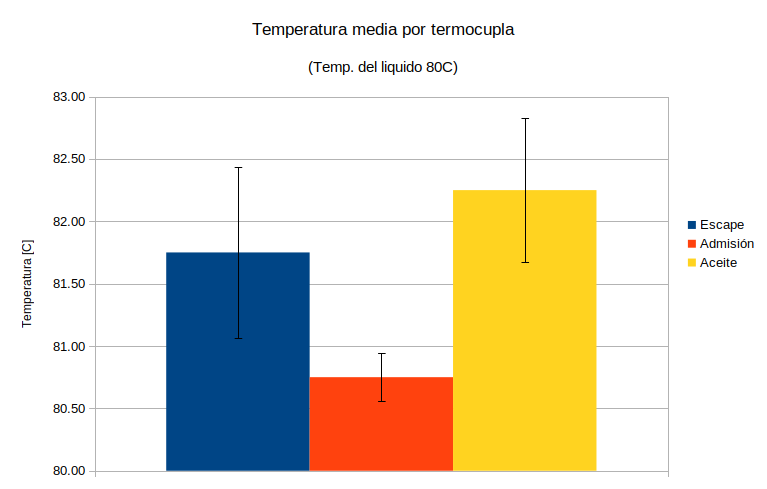
\includegraphics[width=.9\textwidth]{./Figures/temp-80c.png}
\caption{Valores medios y desviación estándar para el ensayo de temperatura a 0C.}
\label{fig:temp-80c}
\end{figure}

El resultado con menor diferencia al valor contrastado fue para la termocupla de temperatura de aceite en el ensayo de 0 \degree C, dicho error fue de 0,25 \degree C. La mayor diferencia se encontró para la termocupla de aceite en el ensayo a 80 \degree C, en ese caso el error fue de 2,25 \degree C. Este error máximo es considerado aceptable para la aplicación del sistema.

\break

\subsection{Ensayos de medición de velocidad de giro}

Para este ensayo se desarrolló, con una placa de desarrollo Arduino MEGA, un simulador de una señal proveniente de un sensor de reluctancia variable. El objetivo del programa desarrollado fue de generar una señal cuadrada periódica, de frecuencia seleccionable, y de ciclo de trabajo positivo de 10\%.

Para verificar la medición del sistema. Se realizaron ocho mediciones de la señal simulada, a distintos valores de R.P.M., y se utilizó un osciloscopio digital, como instrumento de jerarquía para contrastar los resultados obtenidos. Dichos resultados están plasmados en la tabla \ref{tab:ensayo-rpm}. En la figura \ref{fig:foto-rpm} se aprecia ambas placas conectadas entre si, y la forma de onda de la señal generada (en amarillo), y la señal producida por el MAX9924 (en azul) en la pantalla del osciloscopio.

\begin{figure}[htpb]
\centering
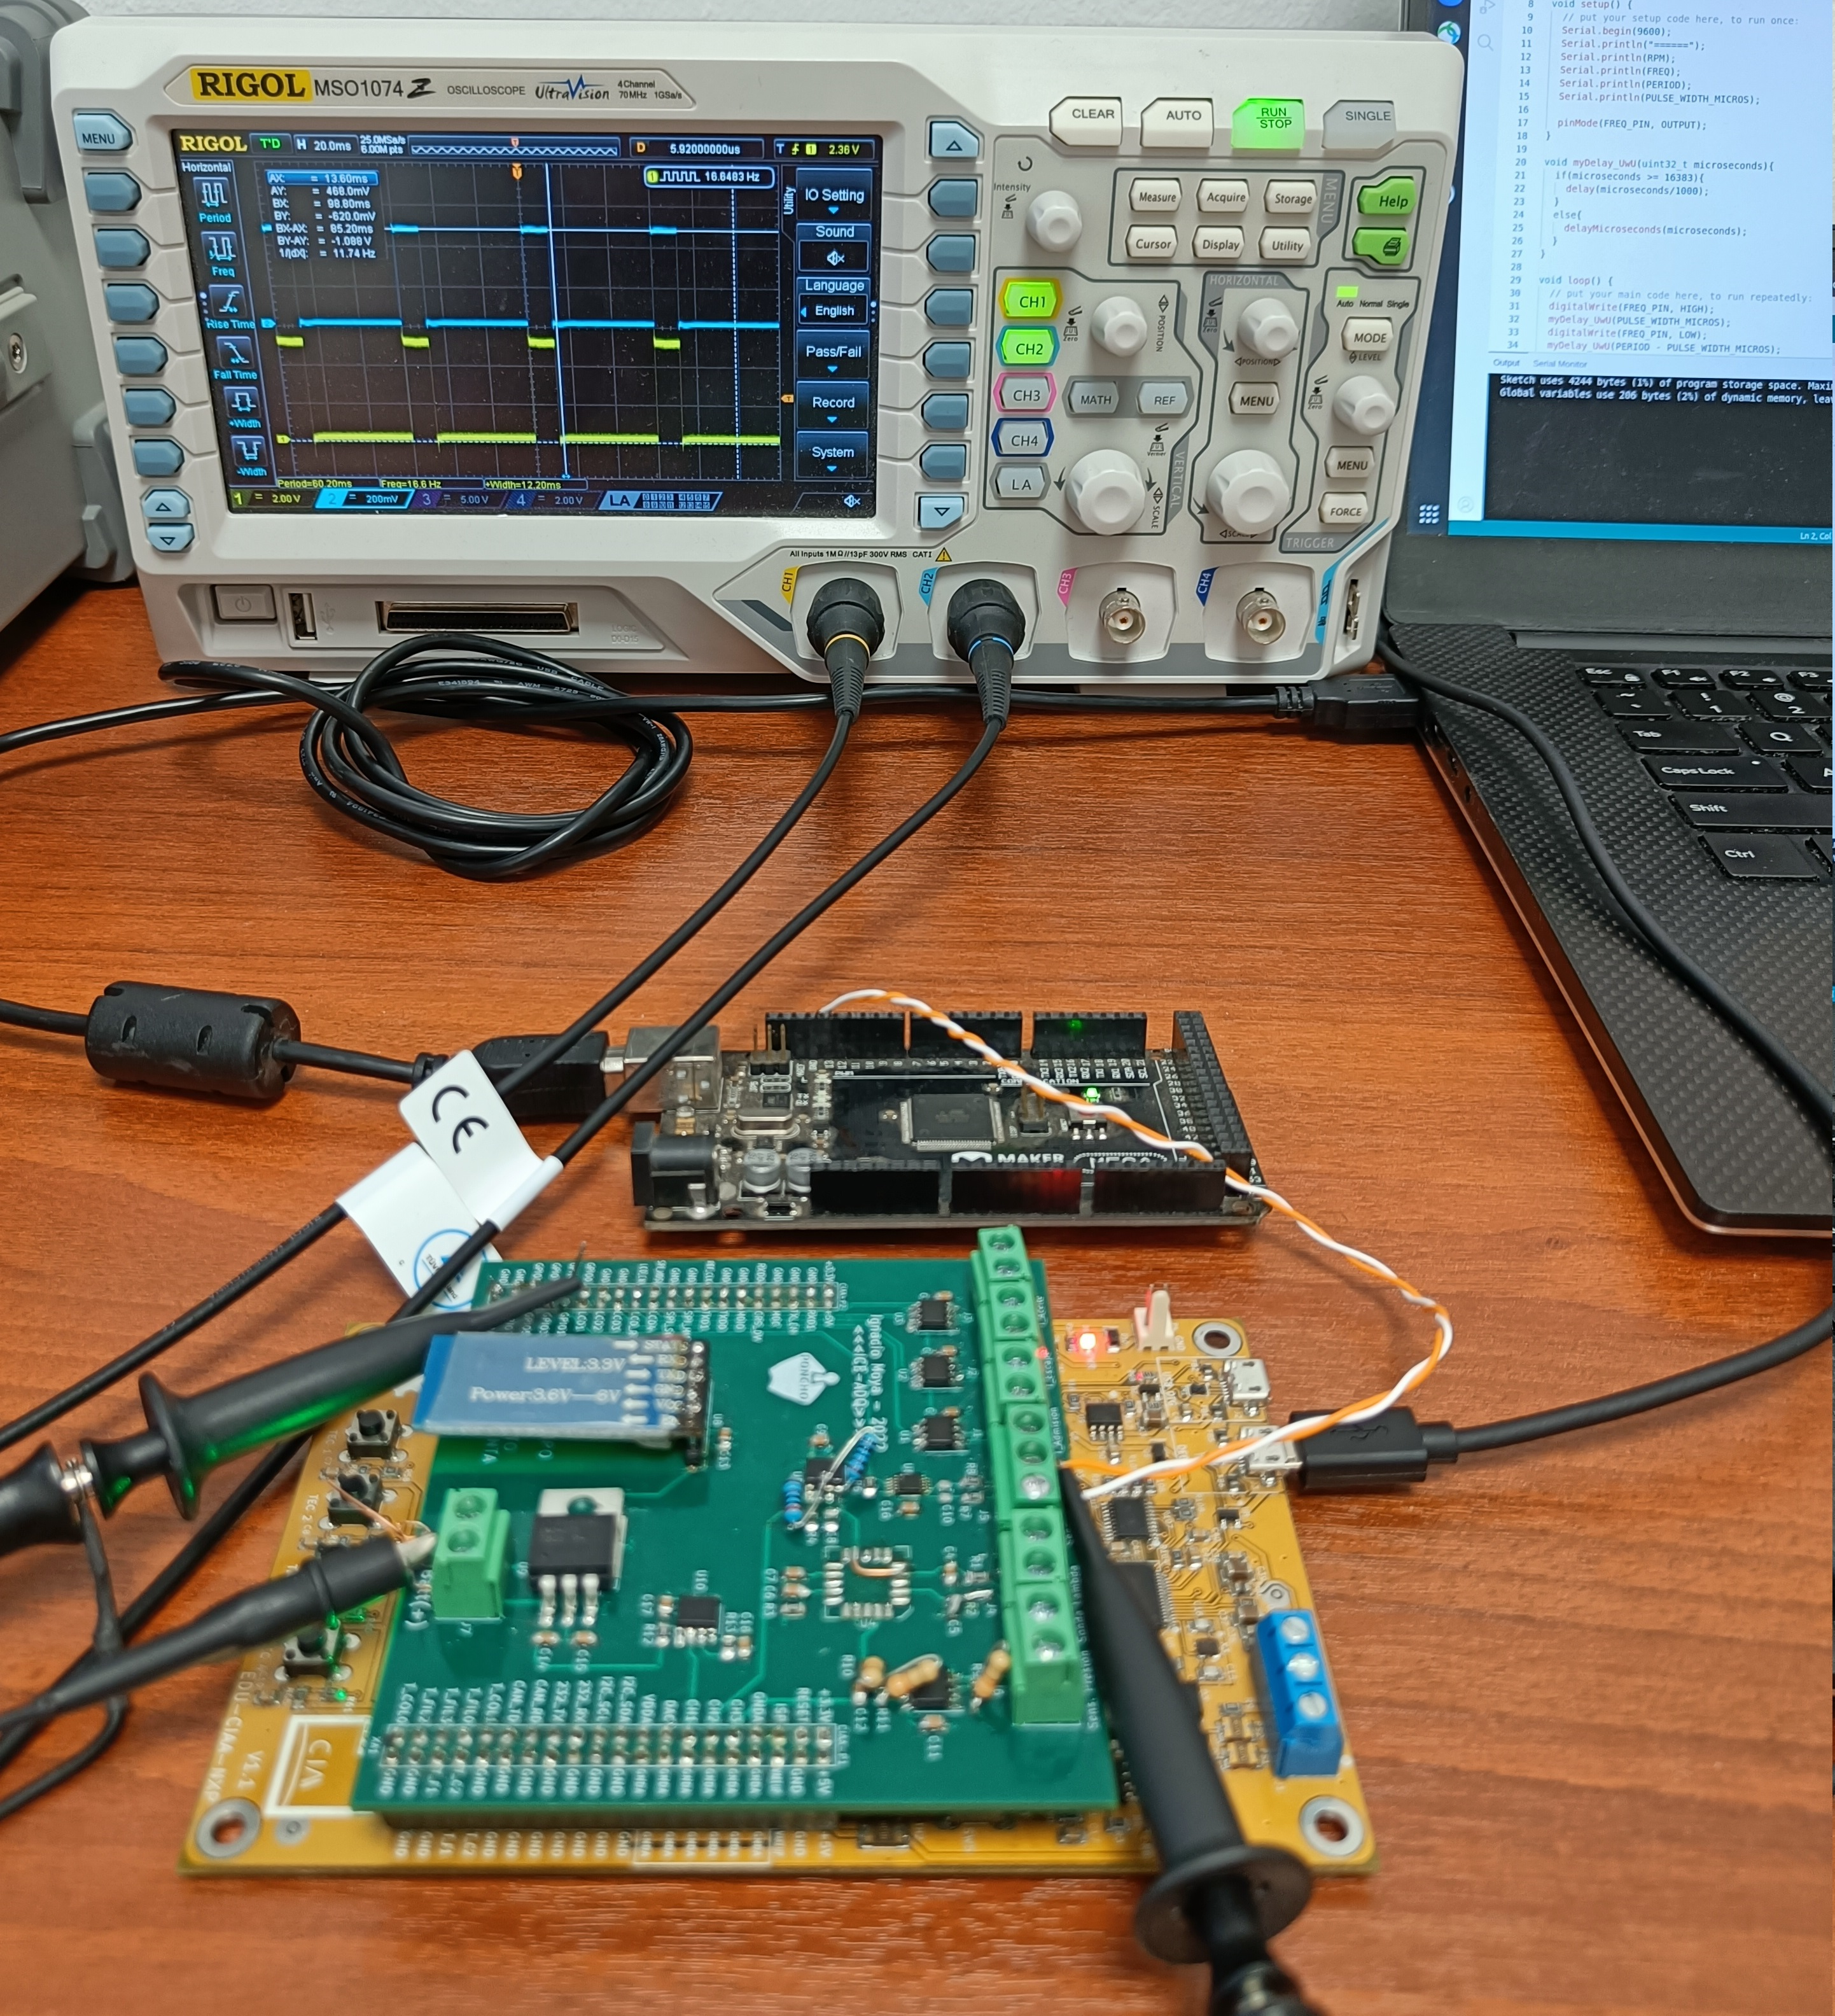
\includegraphics[width=.8\textwidth]{./Figures/foto-rpm.jpg}
\caption{Foto del sistema en funcionamiento conectado a la placa Arduino MEGA utilizada como simulador de señal de R.P.M..}
\label{fig:foto-rpm}
\end{figure}

\begin{table}[htpb]
	\centering
	\caption{Resultados de ensayo de medición de velocidad de giro.}
	\centering
	\begin{tabular}{c c c c}    
		\toprule
		\textbf{Simulada[RPM]} &  \textbf{Referencia[RPM]}   & \textbf{Observada[RPM]} & \textbf{Error[RPM]}\\
		\midrule
		1000	&	998 &	900 & 98\\
		2500	&	2577 & 2400 & 177\\
		5000	&	4967 & 5100 & -133 \\
		7500	&	7447 & 7500 & -53\\
		10000	&	9925 & 9900 & 25\\
		12500	&	12402 & 12300 & 102\\
		15000	&	14876 & 14700 & 176\\
		17500	&	17182 & 17100 & 82\\
		20000	&	19817 & 19800 & 17\\		
		\bottomrule
	\end{tabular}
	\label{tab:ensayo-rpm}
\end{table}

Como se puede observar de los resultados del ensayo. La diferencia máxima entre el valor medido y el contrastado fue de 133 R.P.M., con esto entonces se cumple con el requisito REQ-ADQ-003.

\break

\subsection{Ensayos de medición de presión de aceite}

Para verificar que la medición de presión de aceite cumpliera con el requisito REQ-ADQ-005 se realizaron dos ensayos distintos.

En el primero se simuló al sensor de presión con un potenciómetro de valor similar. Luego se midió la tensión en los contactos de la bornera en donde se conecta el sensor con el circuito impreso. Y, finalmente, se contrastó el valor de tensión medido, con la lectura realizada por el ADC, para ver en cuanto diferían entre si. Los resultados del ensayo están listados en la tabla \ref{tab:ensayo-presion}. El error máximo se dio para el caso de 0,847 V, equivalente a una presión de 66,007 PSI y fue de 0,519 PSI. Dicho error es considerado aceptable. 

\begin{table}[htpb]
	\centering
	\caption{Resultados de ensayo medición de presión de aceite.}
	\centering
	\begin{tabular}{c c c c}    
		\toprule
		\textbf{Tensión[V]} & \textbf{Presión equivalente[PSI]} & \textbf{Lectura[PSI]} & \textbf{Error[PSI]}\\
		\midrule
		0,172		&   5,980 & 5,580 & 0,4 \\
		0,847		&   66,007 & 65,488 & 0,519 \\
		1,429		&   117,764 & 117,418 & 0,346 \\
		\bottomrule
	\end{tabular}
	\label{tab:ensayo-presion}
\end{table}

\subsection{Ensayos de medición de la sonda lambda}

Ante la falta de un dispositivo capaz de leer una sonda lamba para luego contrastar su lectura. Se simuló una sonda Lambda con una fuente de tensión variable digital. Y se realizaron mediciones para 10 valores de tensión, simulando 10 valores distintos de factor lambda. Los resultados de las mediciones pueden verse de la tabla \ref{tab:caso-o2}. El error máximo registrado fue de -, considerado aceptable para la aplicación.

\begin{table}[htpb]
	\centering
	\caption{Resultados de ensayo medición de presión de aceite.}
	\centering
	\begin{tabular}{c c c c}    
		\toprule
		\textbf{Tensión[V]} & \textbf{Lambda equivalente[$\lambda$]} & \textbf{Lectura[$\lambda$]} & \textbf{Error[$\lambda$]} \\
		\midrule
		0,510		&   0,650 & - & - \\
		0,884		&   0,750 & - & - \\
		1,177		&   0,850 & - & - \\
		1,409		&   0,950 & - & - \\
		1,448		&   0,970 & - & - \\
		1,500		&   1,003 & - & - \\
		1,548		&   1,050 & - & - \\
		1,624		&   1,132 & - & - \\
		1,832		&   1,429 & - & - \\
		2,069		&   1,990 & - & - \\
		\bottomrule
	\end{tabular}
	\label{tab:ensayo-o2}
\end{table}

\subsection{Ensayo de pérdida de paquetes}

Para este ensayo se modificó el software de ambas partes del sistema para agregar un campo extra a cada paquete transmitido para enumerar a cada uno de ellos con un número que comienza en 0 y se incrementa por 1 cada vez que se transmite un paquete. De esta forma es posible saber si existió pérdida de paquetes durante la transmisión verificando que la secuencia de los números no se vio interrumpida al finalizar el ensayo. Luego se colocaron ambas partes separadas por una distancia de tres metros y se inició la trasmisión de información hasta llegar a la cantidad de 10.000 paquetes transmitidos. 

Resultado: No se encontró pérdida de datos después de 10.000 transmisiones consecutivas, se verificó que el requisito REQ-COMM-001 fue cumplido.

\subsection{Ensayo de tiempo de transmisión}

Para esta prueba, se modificó el firmware de forma de poder hacer uso de dos de los pines de propósito general disponibles. Uno de ellos se utilizó para indicar, con un valor alto, que la tarea de medición de temperatura está en proceso de adquisición. El pin restante se utilizó para indicar cuando el paquete measurement fue envíado por la tarea de transmisión. Entonces, a través del uso de un analizador lógico, se midió el tiempo entre los cambios de estado de ambos pines. Midiendo así el tiempo que transcurre entre que se obtuvo una medición de la variable hasta que fue transmitida. El resultado de una de estas mediciones puede apreciarse en la figura \ref{fig:tiempo-envio}. El promedio tiempo observado, a partir de tomar diez mediciones consecutivas, fue de 52,2 ms. De esta forma se cumple con el requisito REQ-ADQ-006.

\begin{figure}[htpb]
\centering
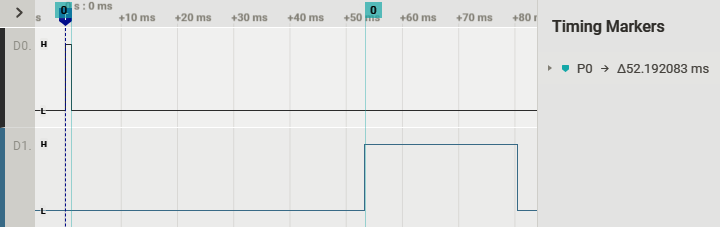
\includegraphics[width=\textwidth]{./Figures/tiempo-envio.png}
\caption{Captura de pantalla del software del analizador lógico, donde se puede apreciar que el tiempo que transcurre entre, adquisición y envío del dato, es de 52 ms aproximadamente.}
\label{fig:tiempo-envio}
\end{figure}

\section{Casos de uso}

En esta sección se describen los casos y las pruebas realizadas para validar, si la interfaz gráfica cumple con sus requerimientos de aceptación. A mismo tiempo, se utilizaron estos ensayos para evaluar si son necesarios cambios o mejoras en el diseño de la interfaz.

Al finalizar estas pruebas se verificó que el diseño y la implementación de la interfaz gráfica es adecuado para sus requisitos. Sin embargo se encontró que la pantalla utilizada era de un tamaño muy pequeño, y esto dificultaba la lectura de las gráficas y la interacción con los botones a través de la interfaz táctil.

\begin{table}[htpb]
	\centering
	\caption{Caso de uso de conectarse a la parte adquisidora.}
	\centering
	\begin{tabular}{c p{0.6\textwidth}}    
		\toprule
		\textbf{Título }     & \textbf{Descripción} \\
		\midrule
		Identificador		&  CU1. \\
		Nombre				&   Conectarse a parte adquisidora. \\
		Actor principal		&   Usuario \\
		Disparadores		&   El usuario presiona el botón \textit{Conectar} \\
		Flujo básico		&   \\
		Pre-condiciones		&   La parte adquisidora tiene que estar funcionamiento y su LED azul parpadeando. \\
		Post-condiciones	&    \\
		\bottomrule
	\end{tabular}
\label{tab:caso-conectar}
\end{table}

\begin{table}[htpb]
	\centering
	\caption{Caso de uso de ocultar una variable de su gráfica.}
	\centering
	\begin{tabular}{c p{0.6\textwidth}}    
		\toprule
		\textbf{Título }     & \textbf{Descripción} \\
		\midrule
		Identificador		&  CU2. \\
		Nombre				&   Ocultar variable en la gráfica. \\
		Actor principal		&   Usuario \\
		Disparadores		&   El usuario presiona el botón que tiene el mismo nombre de la variable que quiere ocultar. \\
\\
		Pre-condiciones		&   La variable se encuentra visible. \\
		Post-condiciones	&   La variable deja de estar visible.\\
		\bottomrule
	\end{tabular}
\label{tab:caso-ocultar}
\end{table}

\begin{table}[htpb]
	\centering
	\caption{Caso de uso de mostrar una variable oculta.}
	\centering
	\begin{tabular}{c p{0.6\textwidth}}    
		\toprule
		\textbf{Título }     & \textbf{Descripción} \\
		\midrule
		Identificador		&	CU3. \\
		Nombre				& 	Mostrar variable oculta. \\
		Actor principal		&   Usuario \\
		Disparadores		&   El usuario presiona el botón que tiene el mismo nombre de la variable que quiere mostrar. \\
\\
		Pre-condiciones		&   La variable se encuentra oculta. \\
		Post-condiciones	&   La variable es visualizada en su gráfica correspondiente.\\
		\bottomrule
	\end{tabular}
\label{tab:caso-mostrar}
\end{table}

\begin{table}[htpb]
	\centering
	\caption{Caso de uso de mostrar una variable oculta.}
	\centering
	\begin{tabular}{c p{0.6\textwidth}}    
		\toprule
		\textbf{Título }     & \textbf{Descripción} \\
		\midrule
		Identificador		&	CU4. \\
		Nombre				& 	Aumentar valor de alarma. \\
		Actor principal		&   Usuario \\
		Disparadores		&   El usuario presiona alguno de los botones \"+\" que se encuentran al lado de los nombres de las variables. \\
\\
		Pre-condiciones		&   Ninguna \\
		Post-condiciones	&   El valor de la alarma se incrementa en una unidad.\\
		\bottomrule
	\end{tabular}
\label{tab:caso-aumentar}
\end{table}

\begin{table}[htpb]
	\centering
	\caption{Caso de uso de mostrar una variable oculta.}
	\centering
	\begin{tabular}{c p{0.6\textwidth}}    
		\toprule
		\textbf{Título }     & \textbf{Descripción} \\
		\midrule
		Identificador		&	CU5. \\
		Nombre				& 	Disminuir valor de alarma. \\
		Actor principal		&   Usuario \\
		Disparadores		&   El usuario presiona alguno de los botones \"-\" que se encuentran al lado de los nombres de las variables. \\
\\
		Pre-condiciones		&   Ninguna \\
		Post-condiciones	&   El valor de la alarma disminuye por una unidad.\\
		\bottomrule
	\end{tabular}
\label{tab:caso-decrementar}
\end{table}

